\documentclass{beamer}
\mode<presentation> 
\usetheme{CambridgeUS}
\usecolortheme{seagull}
%\setbeamertemplate{headline}
%\setbeamertemplate{footline} 
% To remove the footer line in all slides uncomment this line

%\setbeamertemplate{footline}[page number] 
% To replace the footer line in all slides with a simple slide count uncomment this line

\setbeamertemplate{navigation symbols}{} 
% To remove the navigation symbols from the bottom of all slides uncomment this line

\usepackage{graphicx}
%\usepackage{tcolorbox}
\usepackage{booktabs} 
\usepackage[round]{natbib}
\usepackage{verbatim}
\usepackage{subfigure}
\usepackage{multicol}
\newcommand{\beginbackup}{
	\newcounter{framenumbervorappendix}
	\setcounter{framenumbervorappendix}{\value{framenumber}}
}
\newcommand{\backupend}{
	\addtocounter{framenumbervorappendix}{-\value{framenumber}}
	\addtocounter{framenumber}{\value{framenumbervorappendix}} 
}
%----------------------------------------------------------------------
%	TITLE PAGE
%----------------------------------------------------------------------

\title[Narrative Conservatism]{Narrative Conservatism} % The short title appears at the bottom of every slide, the full title is only on the title page
\author[]{Juan Manuel Garc\'ia Lara, Beatriz Garc\'ia Osma, Fengzhi Zhu} % Your name
\institute[] % Your institution as it will appear on the bottom of every slide, may be shorth and to save space
{\textit{\textit{Universidad Carlos III de Madrid}} \\ % Your institution for the title page

	\bigskip
	
\medskip
\large Queen Mary University of London

} % Your email address
\date{\today} % Date, can be changed to a custom date (\today)

\begin{document}
	
\begin{frame}
\titlepage % Print the title page as the first slide
\end{frame}

%-----------------------------------------------------------------
%\begin{frame}
%\frametitle{Outline}
%\tableofcontents
%\end{frame}

%-------------------------------------------------------------------
%	PRESENTATION SLIDES
%----------------------------------------------------
\section{Research Question and Contribution}
%------------------------------------------------

\begin{frame}
\frametitle{Research Question and Contribution}
\begin{itemize}
\item \textbf{Research Question}

\begin{itemize}
\item Is narrative disclosure conservative?

\end{itemize}

\medskip
\pause

\item \textbf{Findings}
\begin{itemize}
\item Using 8-K and 10-Q data (1994-2019), we define and find evidence of narrative conservatism. 
\item Narratives reflect bad news in a more \textbf{complete}, \textbf{news-consistent}, and \textbf{timely} manner than good news.
\end{itemize}

\medskip

\pause

\item \textbf{Contribution}

\begin{itemize}
	\item Extend literature on accounting conservatism by defining and documenting the existence of narrative conservatism.
	\item Explore the links between recognition and narrative disclosure.
	\item Add to the debate on whether managers withhold bad news. 
	\item Add to the broader literature on the informativeness of SEC filings.
\end{itemize}
\end{itemize}
\end{frame}
%------------------------------------------------
\section{Theoretical Framework}
%------------------------------------------------
\begin{frame}
\frametitle{Theoretical Framework: Conservatism}
\begin{itemize}
	
	\item \textbf{Accounting Conservatism}
	
	\begin{itemize}
		
		\item Recognition (\citet{beaverConditionalUnconditionalConservatism2005,ballEarningsQualityUK2005})
			\begin{itemize}
		\item \textit{Conditional}: ``higher degree of verification to recognize good news as gains than to recognize bad news as losses," \citep*[p. 7]{basuConservatismPrincipleAsymmetric1997} leading to earnings that recognize bad news in a timelier and more complete manner than good news.
		\item \textit{Unconditional}: ex ante or news independent. Aspects of the accounting process (measurement and recognition criteria at the inception of assets and liabilities), leading to a persistent understatement of net assets.
		 	\end{itemize}
		\pause
		
		\medskip
		
		\item What role disclosure? 
			\begin{itemize}		
		\item  Prior work focuses on recognition, little is known about conservative disclosure \cite[p.243]{kothariManagersWithholdBad2009}.	
		\item A ``committment to timely disclosure of bad news need not come exclusively through financial statement recognition'' \cite*[p. 73-74]{guayConservativeDisclosure2018}:
			
				
					\end{itemize}
		
	\end{itemize}
	
\end{itemize}
\end{frame}
%------------------------------------------------
\begin{frame}
\frametitle{Theoretical Framework: Recognition and Disclosure (I)}
\begin{itemize}
\item \textbf{Recognition and Disclosure \citep{schipperRequiredDisclosuresFinancial2007}}
	
	\begin{itemize}
		\item Recognition: depictions in numbers with captions on the face of the financial statements
		\item Disclosure: display in the notes and supporting schedules that accompany financial statements
	\end{itemize}

	\pause

\medskip

\item \textbf{Reporting Requirement (FASB, IASB)}

	\begin{itemize}
		\item Recognition: an economic event can be recognized if it satisfies \textit{all}:
		\begin{itemize}
			\item Definition criterion
			\item Measurability criterion
			\item Relevance criterion
			\item Reliability criterion
		\end{itemize}
	

	% First, the item must meet the definition of an element of financial statements (definition criterion). Second, the item must have a relevant attribute measurable with sufficient reliability (measurability criterion). Third, the information about the item must be capable of making a difference in user decisions (relevance criterion). Fourth, the information must be representationally faithful, verifiable, and neutral (reliability criterion).
	\pause
		\item Even if criteria are met, annual reports are \textit{still} annual (low frequency and lack of timeliness)
		\item Disclosure: can be deployed to disclose information that fails to meet certain recognition criteria
	\end{itemize}



\end{itemize}
\end{frame}
%------------------------------------------------
\begin{frame}
\frametitle{Theoretical Framework: Recognition and Disclosure (II)}
\begin{itemize}
	
	\item \textbf{Role of Narratives} 
	
		\begin{itemize}
			\item
			``\textit{Although financial statements have essentially the same objectives as financial reporting, some useful information is better provided by financial statements and some is better provided, or can only be provided, by notes to financial statements or by supplementary information or other means of financial reporting.}'' (FASB 1984, par.7)


	\begin{itemize}
		\item Supplement information that cannot be recognized
		\item Explain/complement/provide details of recognized line items
	\end{itemize}
	\end{itemize}
\medskip
\pause

	\item \textbf{What role narratives in conservative accounting?} 

\begin{itemize}
	\item Strategic disclosure and bad news hoarding \citep[e.g.,][]{kothariManagersWithholdBad2009}.
	\item Timely bad news disclosure ameliorates litigation risk, also associated with narratives \citep[e.g.,][]{rogersDisclosureToneShareholder2011,skinnerWhyFirmsVoluntarily1994,skinnerEarningsDisclosuresStockholder1997}.
\end{itemize}




	
\end{itemize}
\end{frame}
%------------------------------------------------


%------------------------------------------------
\begin{frame}
	\frametitle{Theoretical Framework: Asymmetric Completeness}
	\begin{itemize}
\item \textbf{Completeness}

\begin{itemize}
	\item Completeness implies that disclosure includes all necessary information for a user to understand the underlying economic event.
		\begin{itemize}
		\item Disclosure reduces information asymmetry: lowers CoC and increases liquidity \cite{diamondDisclosureLiquidityCost1991,diamondOptimalReleaseInformation1985,leuzEconomicConsequencesIncreased2000}
	\end{itemize}
	
	\item Good news disclosure may be completer, relative to bad news, to boost performance \citep{teohEarningsManagementUnderperformance1998, langVoluntaryDisclosureEquity2000}.
	\item Bad news disclosure may be completer, relative to good news, to avoid litigation \citep{skinnerWhyFirmsVoluntarily1994, skinnerEarningsDisclosuresStockholder1997}.
\end{itemize}

\medskip
\pause
\begin{block}{H1: Asymmetric Completeness}
	Narrative disclosure is more complete in response to bad news than to good news.
\end{block}


\end{itemize}
\end{frame}
%------------------------------------------------
\begin{frame}
	\frametitle{Theoretical Framework: Asymmetric News-consistency}
	\begin{itemize}
		\item \textbf{News-consistency}
		
		\begin{itemize}
			\item News-consistency implies that disclosure agrees with the underlying economic event in content sentiment. %Specifically, we interpret it as the degree to which firms use positive tone in narrative disclosure in response to good news and negative tone in response to bad news.
			\item Tone influences how information is perceived or processed, and thus it can be employed both to inform or mislead \citep{davisNumbersMeasuringInformation2012, liInformationContentForwardLooking2010, huangToneManagement2014}.
			\item Firms may deploy a uniformly positive (negative) tone in both good and bad news disclosure, resulting in higher news-consistency in good (bad) news disclosure.
		\end{itemize}
		
\medskip
\pause
\begin{block}{H2: Asymmetric News-Consistency}
	Narrative disclosure is more news-consistent in response to bad news than to good news.
\end{block}

		
	\end{itemize}
\end{frame}
%------------------------------------------------
\begin{frame}
	\frametitle{Theoretical Framework: Timeliness}
	\begin{itemize}
		\item \textbf{Asymmetric Timeliness}
		
		\begin{itemize}
			\item Timeliness implies that disclosure is made \textit{in time} to be able to influence users' decisions. 
			\item Managers may delay bad news disclosure to mitigate its negative economic consequences \citep{chambersTimelinessReportingStock1984, niessnerStrategicDisclosureTiming2015, segalAreManagersStrategic2016, brockbankStrategicTiming8K2018}.
			\item Managers may accelerate bad news disclosure due to litigation concerns \citep{skinnerWhyFirmsVoluntarily1994, marinovicNoNewsGood2016}.
		\end{itemize}
		
		
\medskip
\pause
\begin{block}{H3: Asymmetric Timeliness}
	Narrative disclosure is timelier in response to bad news than to good news.
\end{block}

		
	\end{itemize}
\end{frame}
%------------------------------------------------
%\begin{frame}
%	\frametitle{Theoretical Framework: Conservatism Continued}
%	\begin{itemize}
%
%\item \textbf{Is conservatism useful?}
%
%	\begin{itemize}
%		\item Valuation role: provide financial information about the reporting entity that is useful to existing and potential investors, lenders, and other creditors in making decisions about providing resources to the entity \citep[OB2]{fasbConceptualFrameworkFinancial2018b}
%		\item Stewardship role: how efficiently and effectively the entity's management and governing board have discharged their responsibilities to use the entity's economic resources \cite[OB4]{fasbConceptualFrameworkFinancial2018b}
%	\end{itemize}
%
%\item \textbf{Is narrative conservatism useful?}
%	\begin{itemize}
%		\item We posit that narrative conservatism enhances contract efficiency and serves the stewardship role of accounting
%		\item Testable hypotheses to be developed
%	\end{itemize}
%
%\end{itemize}
%\end{frame}
%%------------------------------------------------
\section{Research Design}
%------------------------------------------------
\begin{frame}
\frametitle{Research Design: Proxies}
\begin{itemize}

\item \textbf{Narrative Disclosure Corpora}

	\begin{itemize}
		\item Corpora: 10-Q and 8-K filings because they (a) are more credible, (b) have higher reporting threshold and (c) are more timely than other corporate communication channels.
		\item Heterogeneity between 10-Q and 8-K: (a) 10-Q is more diversified in content (b) 8-K is more timely.
	\end{itemize}

\medskip
\pause

\item \textbf{Proxies for Textual Properties (TEX) and News}
	\begin{itemize}
		\item Completeness (NW): natural logarithm one plus total number of words of SEC filings, also number items (NITEMS) and number of 8-Ks (N8K) \pause
		\item News-consistency (TONE): marginal change of tone in response to  good vs. bad news. TONE is number of net positive words per thousand words. \pause
		\item Timeliness (TLAG): reporting time lag, defined as the number of days elapsed between the news release date and the filing date of the studied disclosure \pause
		\item Good and Bad News (RET): stock returns \citep{basuConservatismPrincipleAsymmetric1997}.
	\end{itemize}

\end{itemize}
\end{frame}
%------------------------------------------------
\begin{frame}
\frametitle{Research Design: Model for 10-Q (I)}
\begin{itemize}
	
	\item \textbf{Model Specification}
	\begin{itemize}
		\item \textbf{Form 10-Q}: We explore  responsiveness to good versus bad news: 
		\begin{equation}
		\begin{aligned} 
		\label{eq1}
		TEX_{i,t}=
		&\beta_0+\beta_1QRET_{i,t}+\beta_2NEG_{i,t}+\beta_3QRET_{i,t}\times NEG_{i,t}+\\
		&\sum\beta_nCONTROLS_{i,t}+\epsilon_{i,t},
		\end{aligned} 
		\end{equation}
		
		
		
		\item QRET quarterly market-adjusted stock return
		\item NEG bad news indicator (1 if QRET negative, 0 otherwise)
		\item CONTROLS: Size, MTB, Leverage, Age, Complexity, profitability, operating risk, analyst earnings forecast errors, readability 
	\end{itemize}
\end{itemize}
\end{frame}
%------------------------------------------------
\begin{frame}
\frametitle{Research Design: Model for 8-K}
\begin{itemize}
	
	\item \textbf{Model Specification}
	\begin{itemize}
	
		\item \textbf{Form 8-K}: we explore responsiveness to good versus bad news.
		\begin{equation}
		\begin{aligned}
		\label{eq2}
		TEX_{i,t}=
		&\beta_0+\beta_1\Delta DRET_{i,t-tlag}+\beta_2BN_{i,t-tlag}+\\
		&\beta_3\Delta DRET_{i,t-tlag}\times BN_{i,t-tlag}+\\
		&\sum\beta_nCONTROLS_{i,t}+\epsilon_{i,t},
		\end{aligned}
		\end{equation}
		
		\pause
				\item $\Delta DRET$ is change in daily returns
				\item BN is bad news day, 1 if $\Delta DRET$ is three times larger than average change in DRET.
		
		\begin{figure}[h]
			\centering
			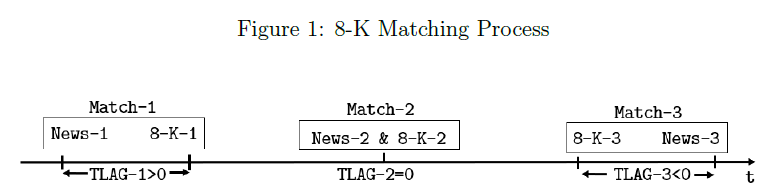
\includegraphics[width=1\linewidth]{fig1}
			\label{fig1}
		\end{figure}
	\end{itemize}
	
\end{itemize}
\end{frame}
%------------------------------------------------
\begin{frame}
\frametitle{Research Design: Data}

\begin{itemize}
	\item US firms period 1994-2019
	\item 8-K and 10-Q files from EDGAR
	\item Data source: Compustat, CRSP and I/B/E/S
	\item Exclude regulated and financial firms
	\item Exclude firms with missing observations

\medskip	\pause
	\item \textit{Final sample 10-Q}: 91,606	observations


\medskip	\pause
	\item \textit{Final sample 8-K}: 119,615	observations	
	\begin{itemize}
	\item If we exclude TLAG over 4 days, sample is 40,700 observations
	\end{itemize}
	
\end{itemize}
\end{frame}
%------------------------------------------------
%\begin{frame}
%\frametitle{Research Design: Data}

%\begin{itemize}
%	\item Data source: Compustat, CRSP and I/B/E/S
	
%	\begin{figure}[h]
%		\centering
%		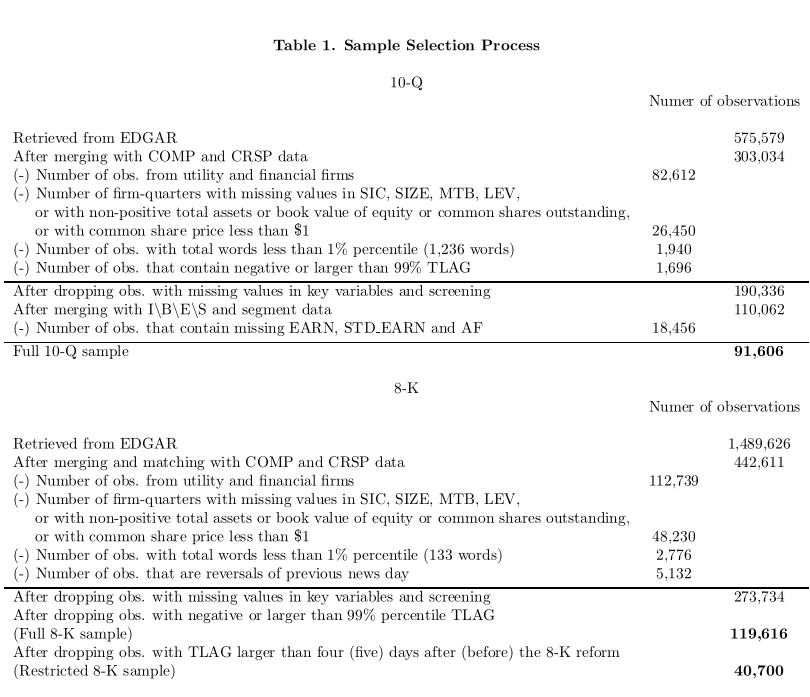
\includegraphics[width=0.7\linewidth]{tab1}
%		\label{tab1}
%	\end{figure}

%\end{itemize}
%\end{frame}
%------------------------------------------------
\section{Results}
%------------------------------------------------
\begin{frame}
\frametitle{Results: Summary Statistics}
\begin{figure}[h]
	\centering
	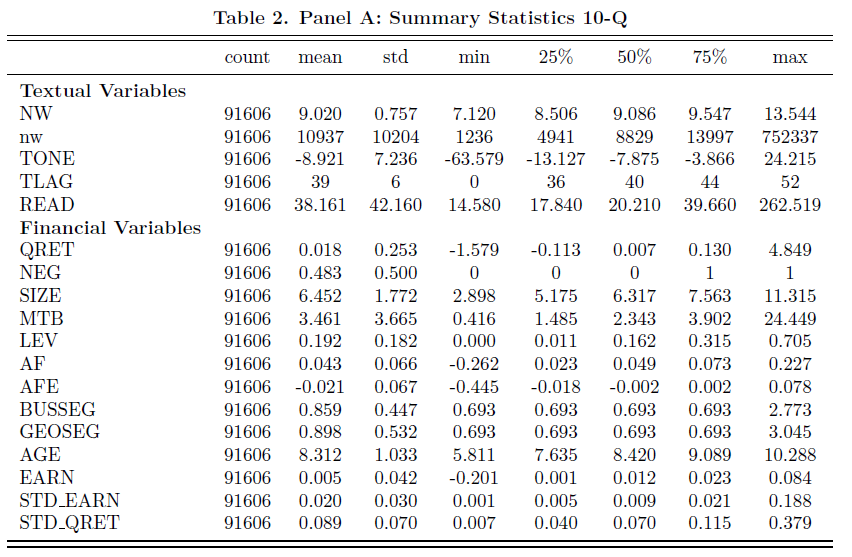
\includegraphics[width=0.9\linewidth]{tab2panA}
	\label{tab2panA}
\end{figure}

\end{frame}
%------------------------------------------------
\begin{frame}
	\frametitle{Results: Summary Statistics Continued}
	\begin{figure}[h]
		\centering
		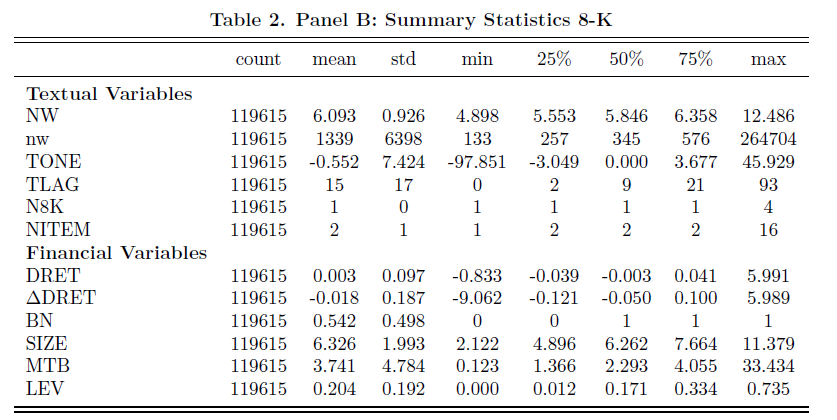
\includegraphics[width=0.9\linewidth]{tab2panB}
		\label{tab2panB}
	\end{figure}
	
\end{frame}
%------------------------------------------------
\begin{frame}
	\frametitle{Results: Summary Statistics Continued}
	\begin{figure}[h]
		\centering
		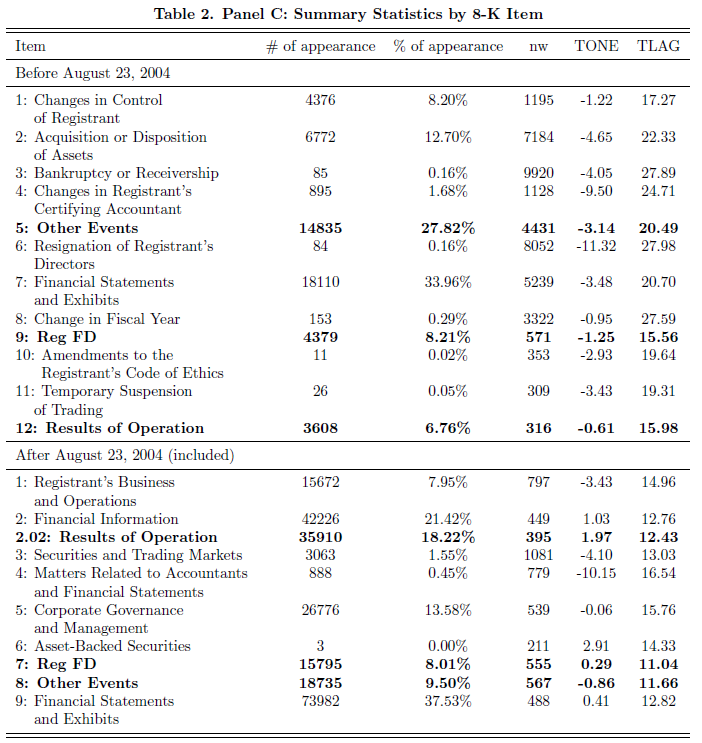
\includegraphics[width=0.6\linewidth]{tab2panC}
		\label{tab2panC}
	\end{figure}
	
\end{frame}
%------------------------------------------------
\begin{frame}
\frametitle{Results: Is 10-Q Narrative Disclosure Conservative?}
	\begin{figure}[h]
		\centering
		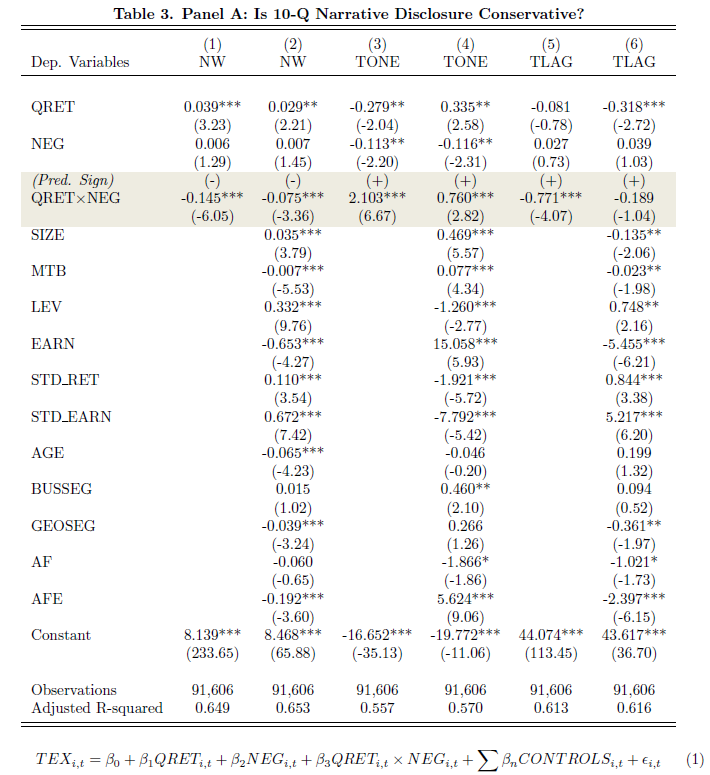
\includegraphics[width=0.9\linewidth]{tab3panA}
		\label{tab3panA}
	\end{figure}
\end{frame}
%------------------------------------------------
\begin{frame}
\frametitle{Results: Are Lengthier 10-Qs Less Readable?}
	\begin{figure}[h]
	\centering
	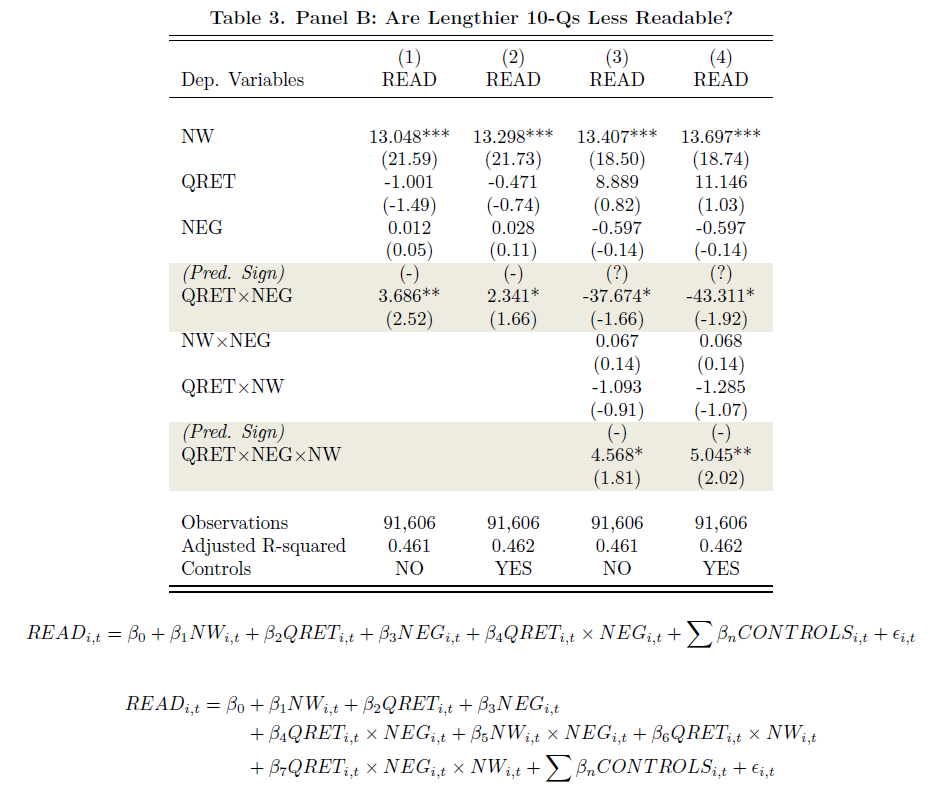
\includegraphics[width=0.9\linewidth]{tab3panB}
	\label{tab3panB}
	\end{figure}
\end{frame}
%------------------------------------------------
\begin{frame}
\frametitle{Results: Is 8-K Narrative Disclosure Conservative?}
	\begin{figure}[h]
	\centering
	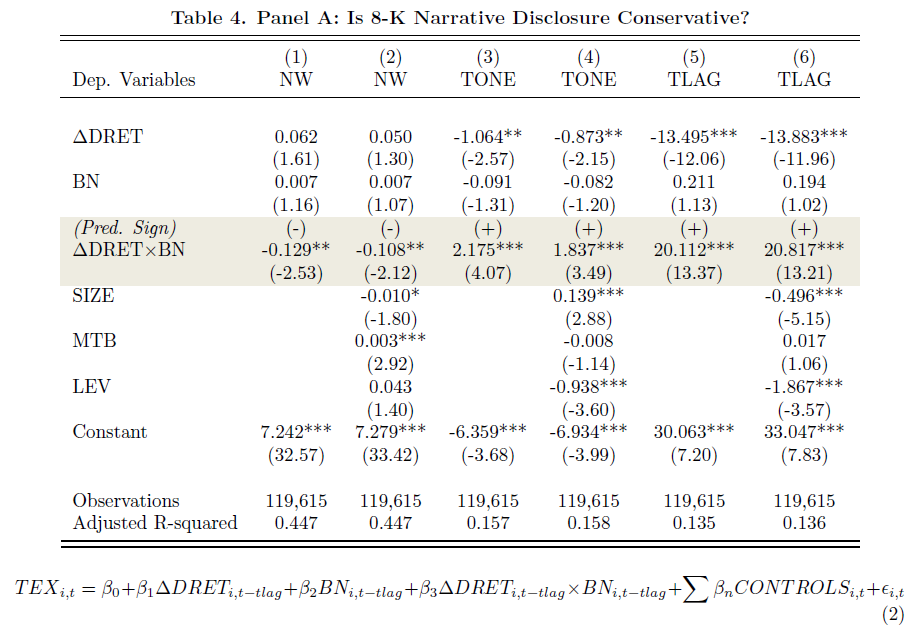
\includegraphics[width=0.9\linewidth]{tab4panA}
	\label{tab4panA}
	\end{figure}
\end{frame}
%------------------------------------------------
\begin{frame}
\frametitle{Results: 8-K Items, Filings and Reporting Time Lag}
	\begin{figure}[h]
	\centering
	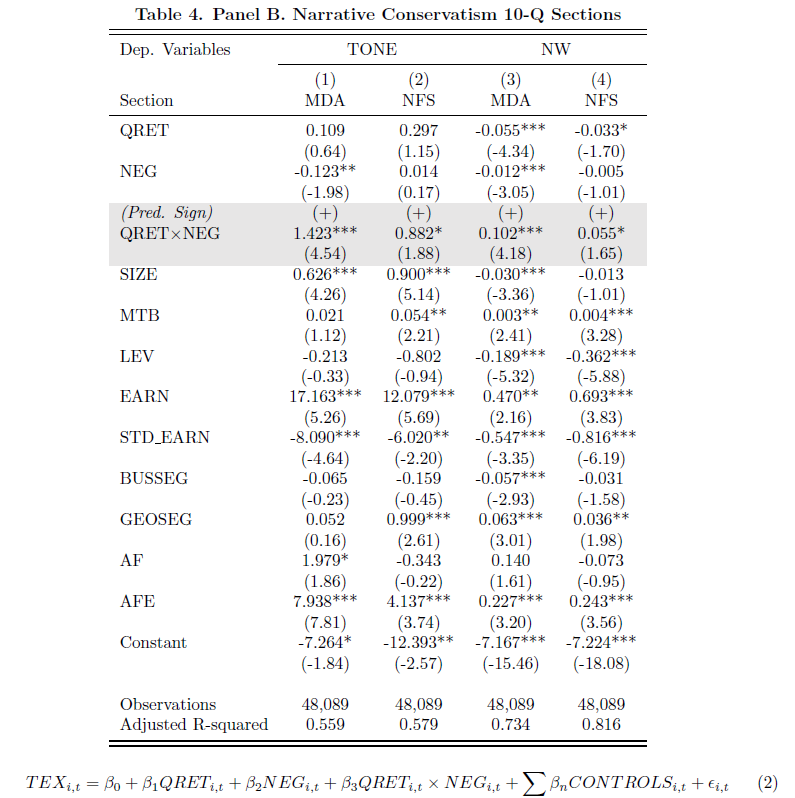
\includegraphics[width=0.9\linewidth]{tab4panB}
	\label{tab4panB}
	\end{figure}
\end{frame}
%------------------------------------------------
\begin{frame}
	\frametitle{Results: Robustness Checks}
\begin{itemize}
	\item Our evidence of narrative conservatism is robust to 
	\begin{itemize}
		\item employing an alternative tone measure using the positive and negative word list from the Harvard General Inquiry dictionary \citep{loughranTextualAnalysisAccounting2016};
		\item including controls for conditional conservatism and managerial incentives;
		\item excluding 8-K items on results of operations that contain quarterly or annual financial statements \citep{segalAreManagersStrategic2016};
		\item using an alternative 8-K reporting time lag definition \citep{carterRelevanceForm8K1999, niessnerStrategicDisclosureTiming2015, chapmanInformationOverloadDisclosure2019};
		\item excluding a priori bad news 8-K items \citep{segalAreManagersStrategic2016};
		\item estimating by fiscal year from 1995 to 2020.
	\end{itemize}
\end{itemize}
\end{frame}
%------------------------------------------------
\section{Additional Analyses}
%------------------------------------------------
%------------------------------------------------
\begin{frame}
\frametitle{Results: Additional Analyses}
\begin{itemize}
	\item We expect to observe greater narrative conservatism
	\begin{itemize}
		\item where managers are more able to have discretion over narrative content: in the MD\&A section as compared to the footnotes;
		\item also, in voluntary disclosures as compared to mandatory disclosures;
		\item in settings where managers have incentives to release bad news
		\item in firms where recognition criteria may be stringer (less opportunities to recognize bad news).
	\end{itemize}
\end{itemize}
\end{frame}
%------------------------------------------------

\begin{frame}
\frametitle{Additional Analyses: MD\&A and NFS}
	\begin{figure}[h]
	\centering
	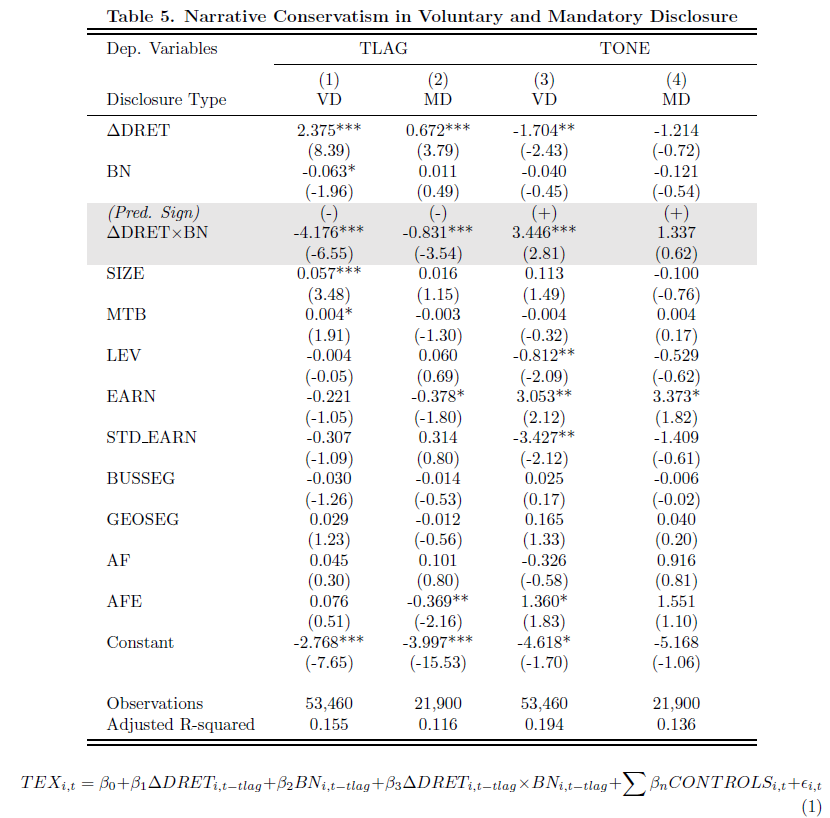
\includegraphics[width=0.9\linewidth]{tab5}
	\label{tab5}
	\end{figure}
\end{frame}
%------------------------------------------------
\begin{frame}
\frametitle{Additional Analyses: Voluntary and Mandatory Disclosure}
	\begin{figure}[h]
	\centering
	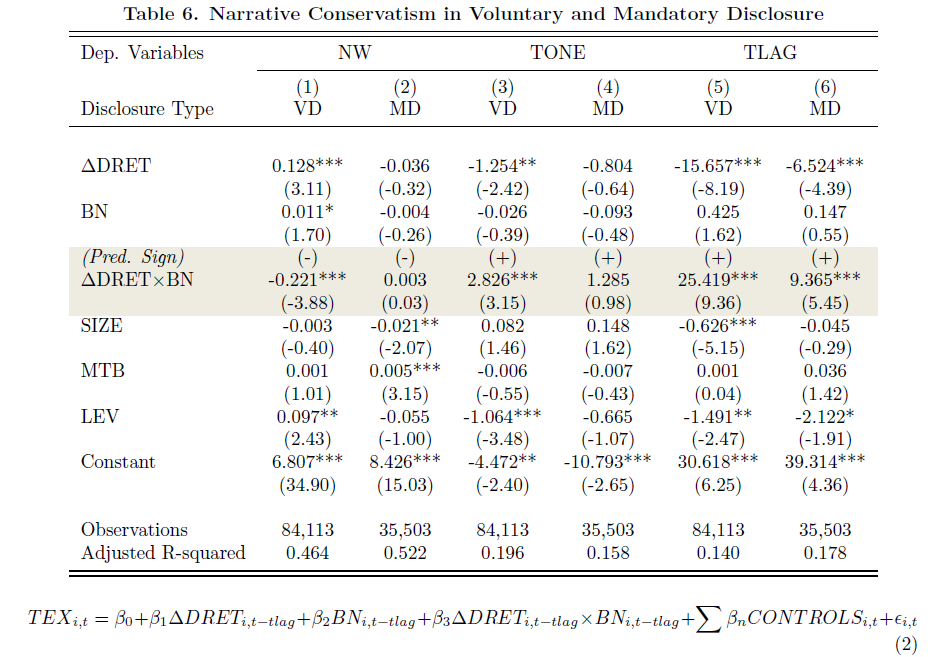
\includegraphics[width=0.9\linewidth]{tab6}
	\label{tab6}
	\end{figure}
	
\end{frame}
%------------------------------------------------
\begin{frame}
	\frametitle{Additional Analyses: Intangible Assets and R\&D Expenses}
	\begin{figure}[h]
	\centering
	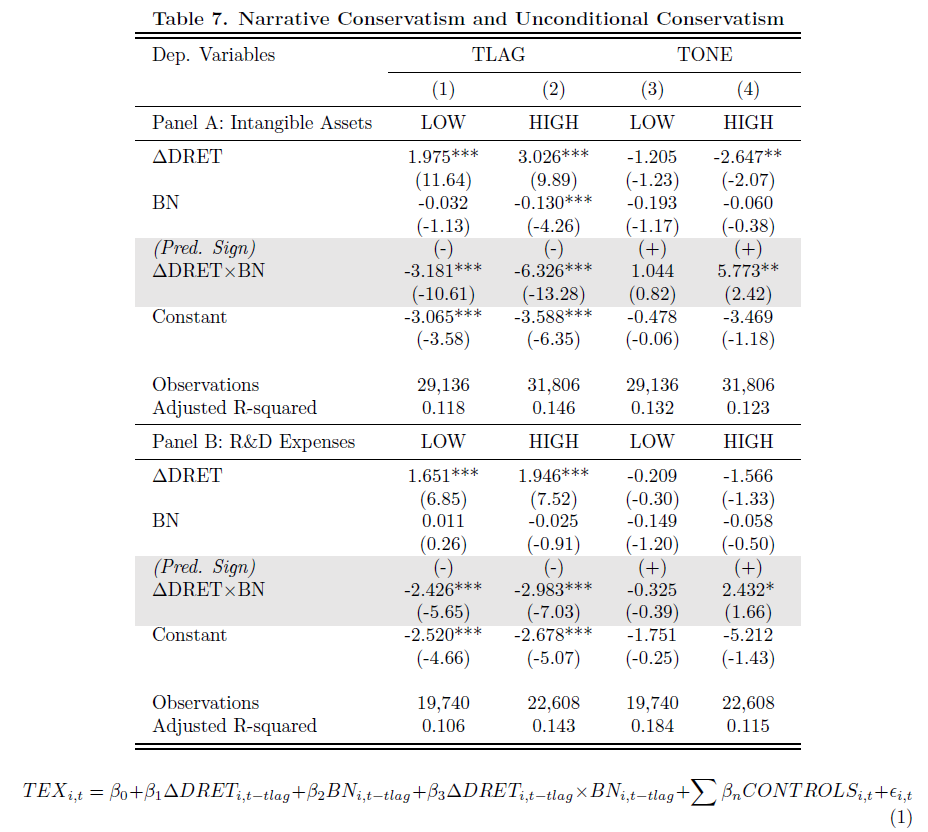
\includegraphics[width=0.9\linewidth]{tab7}
	\label{tab7}
	\end{figure}
	
\end{frame}
%------------------------------------------------
%\begin{frame}
%	\frametitle{Additional Analyses: Firm Characteristics}
%	\begin{figure}[h]
%		\centering
%		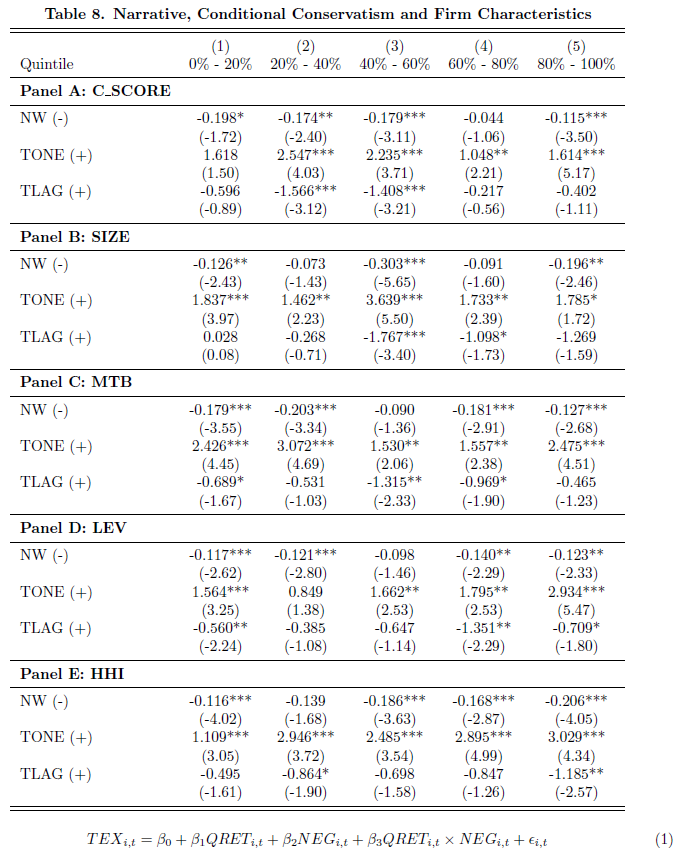
\includegraphics[width=0.65\linewidth]{tab8}
%		\label{tab8}
%	\end{figure}
	
%\end{frame}
%------------------------------------------------
\begin{frame}
	\frametitle{Additional Analyses: Managerial Incentives}
	\begin{figure}[h]
	\centering
	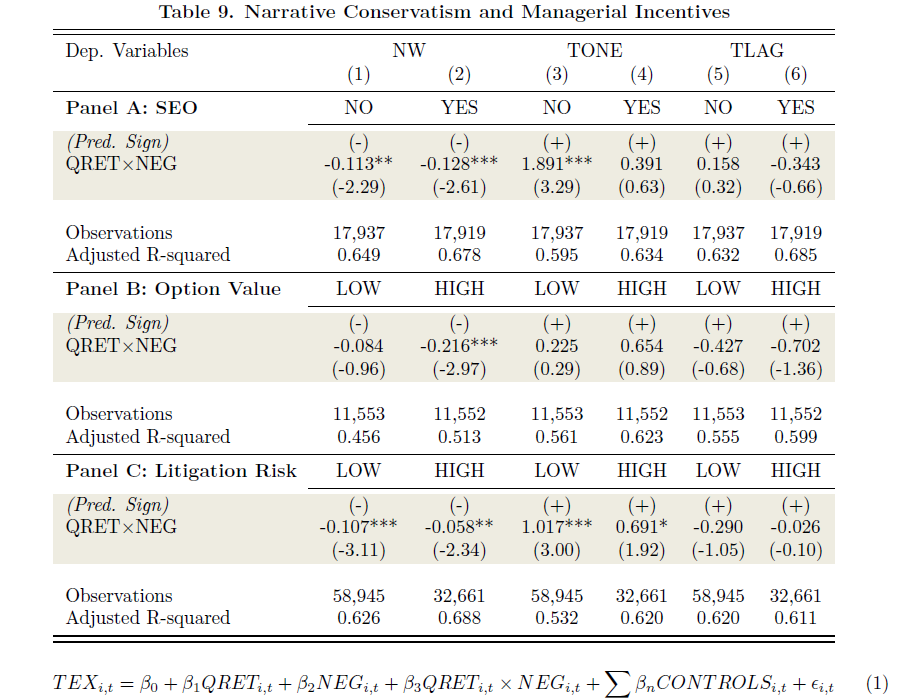
\includegraphics[width=0.8\linewidth]{tab9}
	\label{tab9}
	\end{figure}
\end{frame}
%------------------------------------------------
\section{Conclusions}
%------------------------------------------------
\begin{frame}
\frametitle{Conclusions}
\begin{itemize}
	\item \textbf{Conclusions}
	\begin{itemize}
		\item We provide evidence that narratives reflect bad news in a more complete, news-consistent, and timely manner than good news. 
		\item Firms report lengthier 10-Qs to clarify rather than obfuscate bad news, and provide more 8-Ks and 8-K items in response to bad news than to good news.
		\item We document greater narrative conservatism in the MD\&A section and in voluntary disclosure. Also, narrative conservatism is pervasive in firms with high conditional conservatism, intangible assets, R\&D expenses and proprietary costs.
		\item We find greater narrative conservatism in settings where managers have strong incentives to disclose bad news.
	\end{itemize}


	
\end{itemize}

\end{frame}
%------------------------------------------------
\section{References}
%------------------------------------------------
\beginbackup
\begin{frame}<presentation:0>
\frametitle{Selected References}
\scriptsize
\bibliographystyle{plainnat}
\bibliography{NC_slides}
\end{frame}
\backupend
%------------------------------------------------
\end{document}